\chapter{The Tonnetz and why it is a torus}\label{ch:tonnetz}

\section{Construction as a lattice quotient}
Take the integer lattice $\Z^2$ and the group homomorphism
\[
\varphi:\Z^2\to\Z_{12},\qquad \varphi(i,j)=7i+4j \pmod{12}.
\]
Place lattice point $(i,j)$ in the plane at $i\,\mathbf e_1+j\,\mathbf e_2$ with $\mathbf e_1=(1,0)$ and
$\mathbf e_2=(\tfrac12,\tfrac{\sqrt3}{2})$, and label it with the note $\varphi(i,j)$. Then a step along
$\mathbf e_1$ adds a perfect fifth, a step along $\mathbf e_2$ adds a major third, and a step along
$\mathbf e_1-\mathbf e_2$ adds $7-4=3$, a minor third. Joining each point to its six neighbours triangulates the
plane (\cref{fig:lattice}); this is the layout of the TonnetzViz application \citep{cifka2016} used on the
original slides.

\begin{figure}[t]\centering
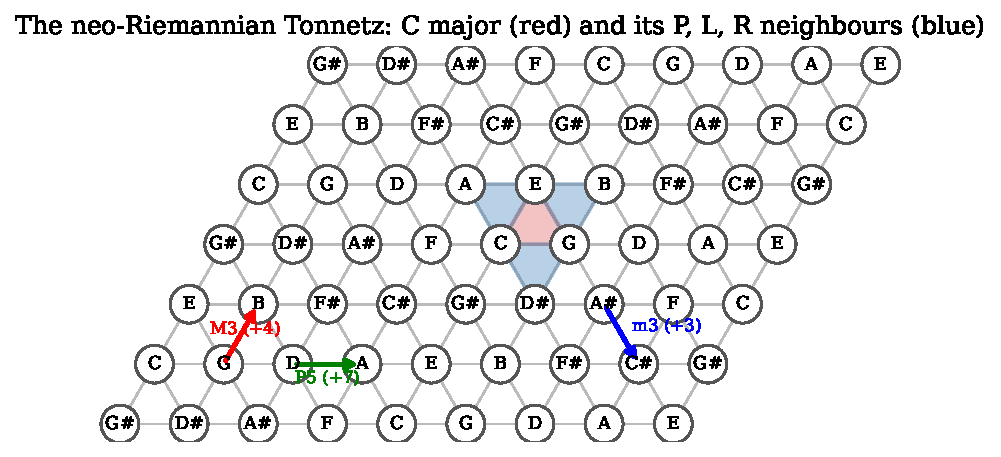
\includegraphics[width=0.86\linewidth]{figures/tonnetz_lattice.pdf}
\caption{The Tonnetz as a labelled triangular lattice. Upward triangles $\{x,x+4,x+7\}$ are major triads;
downward triangles are minor. C major (red) shares an edge with each of Cm, Em and Am (blue): these are its
$P$, $L$ and $R$ neighbours (Chapter~\ref{ch:plr}).}\label{fig:lattice}
\end{figure}

\begin{proposition}\label{prop:triangles}
The upward triangle with lower-left corner $x=\varphi(i,j)$ carries the notes $\{x,x+7,x+4\}$, the major triad on
$x$; the downward triangle on $(i{+}1,j),(i,j{+}1),(i{+}1,j{+}1)$ carries $\{x+7,x+4,x+11\}$, the minor triad on
$x+4$. Every major and minor triad occurs.
\end{proposition}
\begin{proof}
Direct substitution into $\varphi$. Since $\varphi$ is surjective (already $\varphi(i,0)=7i$ runs through all
residues because $\gcd(7,12)=1$), every root $x$ occurs, so every major and every minor triad occurs.
\end{proof}

\section{Identifying equal notes: the torus}
Each note appears infinitely often in the plane. To obtain one copy of each, identify lattice points with equal
labels, i.e.\ form the quotient $\Z^2/\ker\varphi$. The kernel is a sublattice of index 12, and one checks that
\[
\ker\varphi=\{(i,j):7i+4j\equiv0\}=\Z\,(4,-1)\oplus\Z\,(0,3).
\]
Musically, $(0,3)$ says that three major thirds make an octave ($C\to E\to G\sharp\to C$), and $(4,-1)$ that four
fifths up and a major third down return to the start ($C\to G\to D\to A\to E\to C$). The determinant of the basis
is $4\cdot3-(-1)\cdot0=12$, confirming the index.

\begin{theorem}\label{thm:torus}
The quotient of the triangulated plane by $\ker\varphi$ is a torus triangulated with $V=12$ vertices, $E=36$
edges and $F=24$ triangles; $\chi=0$. Its triangles are exactly the 24 major and minor triads.
\end{theorem}
\begin{proof}
A quotient of $\mathbb R^2$ by a rank-2 lattice of translations is a torus (glue opposite sides of the
fundamental parallelogram, \cref{fig:torus}). The lattice triangulation is invariant under the translations,
so it descends. Each vertex has six neighbours (at $\pm3,\pm4,\pm7$, which are six distinct residues), so
$E=12\cdot6/2=36$; each vertex lies in six triangles, so $F=12\cdot6/3=24$. By \cref{prop:triangles} the 24
triangles are the 24 triads, each once. Finally $12-36+24=0$.
\end{proof}

\begin{figure}[t]\centering
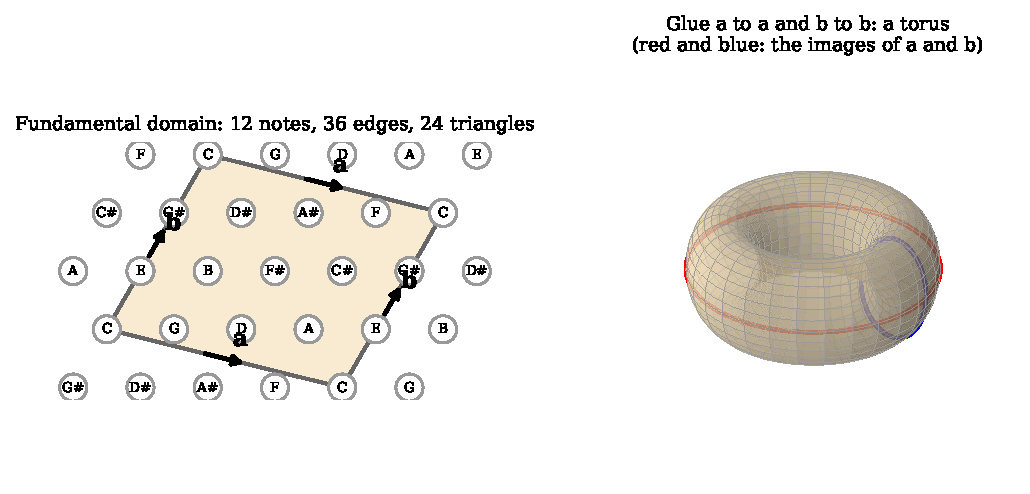
\includegraphics[width=0.92\linewidth]{figures/torus_domain.pdf}
\caption{Left: a fundamental domain spanned by $(4,-1)$ and $(0,3)$; all four corners are C. Gluing edge $a$
to $a$ and $b$ to $b$ (right) yields the torus.}\label{fig:torus}
\end{figure}

A computer check of \cref{thm:torus} is one line of \code{tonnetzkit}:
\begin{lstlisting}
K = generalized_tonnetz(3, 4, 5)   # all T/I images of {0, 3, 7}
K.summary()   # V=12, E=36, F=24, chi=0, betti (1,2,1), orientable -> torus
\end{lstlisting}
The Betti numbers $(1,2,1)$ are those of the torus: one component, two independent loops (the $a$- and
$b$-circles), one enclosed 2-cycle.

\begin{correctionbox}
The slide ``Hamiltonian cycles on a torus'' says the Tonnetz becomes a torus ``when you do octaves''. Octave
equivalence alone is not enough: in just intonation, as Harte, Sandler and Gasser point out, the Tonnetz is an
infinite plane even when octaves are ignored \citep{harte2006}. What closes the plane into a torus is
\emph{pitch-class} equivalence in 12-TET, which additionally equates enharmonic spellings. In particular three
pure major thirds ($5/4)^3=125/64$ fall short of an octave; only in equal temperament do they close exactly.
\end{correctionbox}

\section{Reading chords and progressions}
Because transposition $T_n$ acts on the lattice by translation, any chord or melody has a \emph{shape} on the
Tonnetz that is unchanged by transposition: all major triads are upward triangles and all minor triads downward.
Inversion $I_n$ acts by a point reflection, which is why it swaps the two triangle orientations. A progression
becomes a path of triangles; progressions whose consecutive chords share an edge move by one voice, and
progressions that ``jump'' across the diagram involve larger voice leading.

\paragraph{Other layouts.} Replacing $\varphi$ by $7i+3j$ (fifths and minor thirds) gives a mirror-image drawing of
the same complex, because the three generating intervals $\{3,4,5\}$ are unchanged. Genuinely different Tonnetze
arise only from different trichords (Chapter~\ref{ch:topology}) or from higher-dimensional lattices, for instance
Gollin's three-dimensional Tonnetz for seventh chords \citep{gollin1998}.

\begin{notebookbox}
\sheet{02\_tonnetz\_torus.ipynb}: print the lattice, find the kernel vectors by brute force, and verify
\cref{thm:torus}.
\end{notebookbox}

\begin{qa}
\Qu{Starting from C, which note is reached by the lattice step $(2,1)$?}
\A{$\varphi(2,1)=14+4=18\equiv6$, i.e.\ F$\sharp$: two fifths (C$\to$G$\to$D) and a major third (D$\to$F$\sharp$).}
\Qu{Explain in musical terms why $(0,3)\in\ker\varphi$.}
\A{Three consecutive major thirds, C--E--G$\sharp$--C, return to the starting pitch class (in 12-TET).}
\Qu{Why does each vertex of the Tonnetz have exactly six neighbours?}
\A{Its neighbours are at intervals $\pm3,\pm4,\pm7$, i.e.\ $3,9,4,8,7,5$: six distinct pitch classes.}
\Qu{Compute $\chi$ from the f-vector and name the surface.}
\A{$12-36+24=0$; the complex is orientable, so by \cref{thm:classification} it is the torus.}
\Qu{A student claims the Tonnetz is a sphere because ``it has no edges''. What is wrong?}
\A{Having no boundary does not determine the surface. Both the sphere and the torus are closed; the Euler
characteristic ($0$, not $2$) and the two independent loops ($b_1=2$) show it is a torus.}
\Qu{Why is every major triad an upward triangle?}
\A{Transposition acts by translation and preserves orientation; C major is upward, and every major triad is a
transposition of it.}
\end{qa}
